\chapter{Introduction}
Electricity price forecasting attempts to deduce in advance what the price of electricity will be.
This is a difficult task, as many factors interfere with it: raw materials (as natural gas, coal or uranium) prices, weather conditions or energy demand.
Apart, the local and global economic situation or tax policies and regulations approved by the government affect, among others.

In this Master's Thesis we want to perform forecasts of the energy price in the short, medium and long term, studying which variables affect the price in the Spanish market.
Today, after the covid crisis of previous years and the war in Ukraine, prices have been greatly altered, reaching values that have never been seen before.
In this situation, the completion of this Thesis makes a lot of sense, as we may discover how the market has changed after these two events.

To achieve our goal we will first select the variables that we need to perform the study, download historical data related with them and apply time series analytics tools, both statistical and machine learning based, to understand the data and make forecasts.


\section{The Spanish wholesale electricity market}
In this section we briefly describe how the wholesale electricity market works in Spain.
In 1998, the current regulation came into operation, replacing the previous system in which Red Eléctrica de España (REE) and the Ministry of Industry and Energy entirely planned their transactions.

It allowed the private sector to freely plan the construction of generation plants and the possibility of bidding energy prices, and created the figure of energy supplier (being the consumer able to choose one).
Distribution of energy remained regulated by the government, who assigns this task to a unique company per region. \cite{mercado-electrico-mincotur}

The wholesale electricity market differs from the retail market. In the former generators sell energy to suppliers, while in the latter suppliers sell energy to consumers. Different agents participate in both, and they are regulated by different rules, being more flexible in the retail market.

\subsection{Main agents}
Different agents conform this complex system. Each one is in charge of a specific task:\cite{mercado-electrico-endesa, organismos-reguladores-holaluz}

\begin{itemize}
    \item \textbf{Generators} produce energy and should build, operate and maintain the power plants.
    \item \textbf{Transporters} take the energy from the power plants to the distribution network, building and maintaining the transport network. This network operates in high voltage, making transmission through long distances more efficient.
    \item \textbf{Distributors} extract the energy from the transport network and supply it to the final consumers. They are in charge of building and maintaining the distribution network.
    \item \textbf{Suppliers} buy the energy to generators and sell it to final consumers.
    \item \textbf{Regulators} are in charge of legislating (government administration) and ensuring effective competition (Comisión Nacional de los Mercados y la Competencia, CNMC) in the energy market.
    \item There exist two \textbf{operators}, the market operator and the system operator. The former (Operador de Mercado Ibérico de Energía, OMIE) manages the day-ahead and intraday electricity markets. The latter (Red Eléctrica de España, REE) ensures the system stability, checking that generation and consumption are balanced every time as energy can't be stored in large scale, preventing lack of supply or overload on the power grid. Both operators should work closely, so they can face adequately to problems in the system.
\end{itemize}

\subsection{Main electricity generation technologies}
Energy generation involves the transformation of sources of primary energy into electricity.
The generation technologies differ in the way they produce the energy and in the primary energy they use for this task, each having different building and operation costs, technical characteristics and impact in the environment. \cite{subasta-electrica-totalenergies}


\subsection{The electricity price}
The main goal of this Thesis is to study day-ahead electricity market prices.
These are the prices which supplying companies pay for the energy, and not the final price each consumer pays when using the (Precio Voluntario Pequeño Consumidor, PVPC) tariff, which also includes regulated costs and taxes. \cite{mercado-electrico-xataka}

The prices for next day are fixed in the electricity market or pool.
On it, suppliers make their purchase bids, which are ordered by their value in the supply curve.
On the other hand, generators make their sell bids which are ordered in the demand curve.

\begin{figure}[H]
\centering
    \caption{Energy supply and demand curves in the wholesale market. \cite{curva-oferta-demanda}}
    \label{fig:supply-demand-curves}
    \fbox{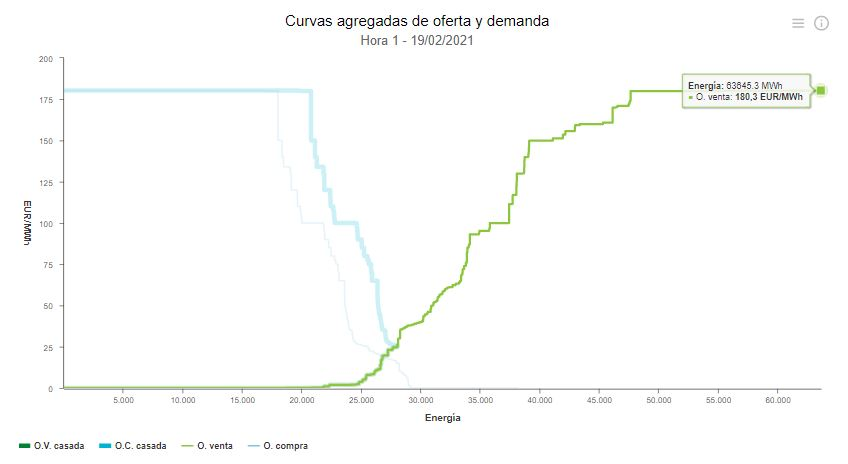
\includegraphics[scale=0.6]{images/supply-demand-curves.jpeg}}
\end{figure}

See figure \ref{fig:supply-demand-curves}: the point where the two curves intersect defines the price at which energy will be sold. On the left of this intersection appear the transactions that will take place, while those on the right will not be materialized, as the generators ask for more money than what suppliers are willing to pay.
All the sold electricity will be available at that intersection price, the generators will receive that price even if they bid for less.

These characteristics are what define a marginal pricing market.
This process will be repeated for each hour of the following day, having a total of 24 different prices.

\subsection{Variables influencing the price}
As the price is built in the free market, defining a model explaining it is very difficult.
Many factors can affect its value, even companies strategic decisions that can't be predicted, but there are some variables that clearly could fit in the equation: \cite{mercado-electrico-periodico-energia, mercado-electrico-cambio-energetico}

\begin{itemize}
    \item \textbf{Demand:} The energy consumption can affect the price, specially in a marginal pricing market. As generation bids are ordered in the supply curve from cheaper to expensive, if the demand is high the intersection point will probably move to the right leading to a higher price.
    \item \textbf{Generation:} Demand and generation are very correlated, as the system operator is in charge of maintaining a balance between both. There are generation technologies that always bid for a low price, even zero, as the nuclear: this is because a nuclear plant can't stop working, so it is always interested in selling the energy no matter the price. Other as wind energy are also sold at a low price but not as low, because it is a cheap energy (the fuel is the own wind) but the more you use a turbine, the more maintenance it needs. As it can be stopped, sometimes is more adequate to do that than selling for zero. The technologies that tend to set the price of electricity are those using commodities as fuel, as combined cycles, because they are the most expensive.
    \item \textbf{Price of commodities:} As the technologies using commodities to make energy usually set the market price, the price of these commodities could be also affecting it. We will study the influence of coal and gas.
    \item \textbf{EU Allowances:} The use of technologies producing carbon emissions requires to pay taxes to the European Union. Companies buy allowances to be able to emmit $CO_2$ and they can trade with them. That's why allowances have market value and it can influence the cost of energy.
    \item \textbf{Time of day/week:)} Something to consider is the moment in time for which we are forecasting. The price is not the same during the day or night, or in weekdays or weekends. This is correlated with the demand and the availability of renewable energy generation.
    \item \textbf{Macroeconomic variables:} The economic situation affects prices, and therefore it can affect electricity cost. GDP or inflation could be potential indicators to study.
\end{itemize}